\documentclass[usenames,dvipsnames]{beamer}
\usepackage{amsmath}
\usepackage{mathtools}
\usepackage{graphicx}
\usepackage{enumitem}
\usepackage{tikz}
\usepackage{gauss}
\usetheme{metropolis}
\usefonttheme[onlymath]{serif}
\title{A Tropical Mindset}
\date{29 April 2018}
\author{Alice McKean}
\institute{Reed Math 201}

\newcommand{\textbs}[1]{{\sffamily\fontseries{sbc}\selectfont #1}}

\newcommand{\mathbs}[1]{\ensuremath{\text{\textbs{#1}}}}
\renewcommand{\mathtt}[1]{\ensuremath{\texttt{#1}}}

\newcommand{\mrs}[1]{\ensuremath{\mathnormal{#1}}} % Reset font to normal
\newcommand{\mbf}[1]{\ensuremath{\mathbf{#1}}}     % Boldface
\newcommand{\mbs}[1]{\ensuremath{\mathbs{#1}}}     % Bold + sans-serif
\newcommand{\mbb}[1]{\ensuremath{\mathbb{#1}}}     % Blackboard bold
\newcommand{\mtt}[1]{\ensuremath{\mathtt{#1}}}     % Teletype
\newcommand{\mrm}[1]{\ensuremath{\mathrm{#1}}}     % Serif ("roman")
\newcommand{\msf}[1]{\ensuremath{\mathsf{#1}}}     % Sans-serif
\newcommand{\msc}[1]{\ensuremath{\mathsc{#1}}}     % Small-caps
\newcommand{\mcl}[1]{\ensuremath{\mathcal{#1}}}    % Calligraphic
\newcommand{\msr}[1]{\ensuremath{\mathscr{#1}}}    % Script
\newcommand{\mfr}[1]{\ensuremath{\mathfrak{#1}}}   % Fraktur

\newcommand{\pic}[2]{\includegraphics[width=#1\columnwidth]{#2}}

\graphicspath{
  {resources/}
}

\newcommand{\minF}[1]{\ensuremath{\text{min}\{ \, #1 \, \}}}

\begin{document}

\maketitle

\begin{frame}{The Shortest Path Problem}
  \begin{figure}
    \pic{1}{shortest-path.png}
  \end{figure}
  % \begin{columns}
  %   \begin{column}{0.6\textwidth}
  %     \begin{figure}
  %       \pic{1}{shortest-path.png}
  %     \end{figure}
  %   \end{column}
  %   \begin{column}{0.4\textwidth}
  %     \begin{align*}
  %       \begin{gmatrix}[p]
  %           0      & 4      & 2      & \infty & \infty & \infty \\
  %           \infty & 0      & 5      & 10     & \infty & \infty \\
  %           \infty & \infty & 0      & \infty & 3      & \infty \\
  %           \infty & \infty & \infty & 0      & \infty & 11     \\
  %           \infty & \infty & \infty & 4      & 0      & \infty \\
  %           \infty & \infty & \infty & \infty & \infty & 0      
  %       \end{gmatrix}
  %     \end{align*}
  %   \end{column}
  % \end{columns}
  \begin{align*}
    D_{u v}^n =\text{min}_{(k, v) \in E}(D_{u k}^{n-1} + D_{k v}^1)
  \end{align*}
\end{frame}
\section{Let's Take a Vacation}
\begin{frame}{The Tropical Semiring}
  The \textit{tropical semiring} is the semiring
  $(\mbb{R} \cup \{ \infty \}, \oplus, \odot)$ where:
  \begin{align*}
    x \oplus y  &= \minF{x, \, y} \\
    x \odot y &= x +_{\mathbb{R}} y \\
    0 &= \infty \\
    1 &= 0_{\mathbb{R}}
  \end{align*}
  As these operations form a semiring they obey various standard properties like
  associativity, commutativity, and distributivity.
\end{frame}
\begin{frame}{Examples}
\begin{align*}
  % 3 \odot 2 \oplus 2 \odot 5
  % &= \minF{ 3 \odot 2, \, 2 \odot 5} \\
  % &= \minF{ 3 +_{\mathbb{R}} 2, \, 2 +_{\mathbb{R}} 5} \\
  % &= \minF{ 5, \, 7 } = 5 \\
  % {} \\
  \infty \oplus 6 &= \minF{ \infty, \, 6 } = 6 \\
  {} \\
  \infty \odot 6 &= \infty +_{\mathbb{R}} 6 = \infty
\end{align*}
It's very important to note that there are no additive inverses.
There does not exist some $x$ such that:
\begin{align*}
  5 \oplus x = \minF{ 5, x } = 0 = \infty
\end{align*}
\end{frame}
\begin{frame}{Freshman's Dream}
  The freshman dream is often stated as $(a + b)^2 = a^2 + b^2$. These poor
  freshmen are just thinking tropically.
  \begin{align*}
    (a \oplus b)^{\odot 2} = a^{\odot 2} \oplus b^{\odot 2}
  \end{align*}
  % \begin{align*}
  %   (a \oplus b)^{\odot 2}
  %   &= (a \oplus b) \odot (a \oplus b) \\
  %   &= a \odot (a \oplus b) \oplus b \odot (a \oplus b) \\
  %   &= a \odot a \oplus a \odot b \oplus b \odot a \oplus b \odot b \\
  %   &= \minF{ a \odot a, \, a \odot b, \, b \odot a, \, b \odot b } \\
  %   &= \minF{ 2a, \, a + b, \, b + a, \, 2b } \\
  %   &= \minF{ 2a, \, 2b } \\
  %   &= \minF{ a \odot a, \, b \odot b } \\
  %   &= (a \odot a) \oplus (b \odot b) \\
  %   &= a^{\odot 2} \oplus b^{\odot 2}
  % \end{align*}
  In fact this pattern holds in general:
  \begin{align*}
    (a \oplus b)^{\odot n} = a^{\odot n} \oplus b^{\odot n}
  \end{align*}
\end{frame}
\begin{frame}{Quick Tell Harvard}
  \begin{figure}
    \pic{1}{lil-pump.jpg}
  \end{figure}
\end{frame}
\begin{frame}{Think Tropically}
  You already solved this problem in your homework:
  \begin{align*}
    \sum_{k=1}^np(i,k,\ell - 1)p(k,j,1)
    &\rightsquigarrow \bigoplus_{k=1}^{n} p(i,k,\ell - 1)\odot p(k,j,1) \\
    &= \kern0.2em \text{min}_{\, k \in V} \left \{ \: p(i, k, \ell - 1) + p(k, j, 1) \, \right \}
  \end{align*}
  For any graph $G$ using a modified adjacency matrix $A = A(G)$ you can find
  the shortest path using $n$ steps with $A^{\odot n}$.
  % For any graph $G$ using a modified adjacency matrix $A = A(G)$ you can solve all pairs shortest
  % path with $A^{\odot | V |}$

  Where $A^{\odot n}$ is matrix exponentiation with tropical matrix multiplication.
\end{frame}
\begin{frame}{Example}
  \begin{figure}
    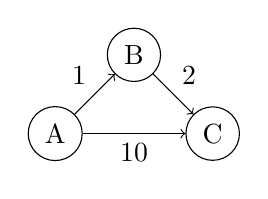
\begin{tikzpicture}
      \draw
      (0,0) node[circle, black, draw](a){A}
      (1,1) node[circle, black, draw](b){B}
      (2,0) node[circle, black, draw](c){C};
      \draw[->] (a) -- node[above,xshift=-0.2cm]{1} (b);
      \draw[->] (a) -- node[below]{10}              (c);
      \draw[->] (b) -- node[above,xshift=0.2cm]{2}  (c);
    \end{tikzpicture}
  \end{figure}
  \begin{align*}
    {
      \rowarrowsep=-7pt
      \begin{gmatrix}[p]
        0      & 1      & 10 \\
        \infty & 0      & 2  \\
        \infty & \infty & 0
      \end{gmatrix}
    }^{\odot2}
    &= 
    \rowarrowsep=-2pt
    \begin{gmatrix}[p]
      0      & 1      & 10 \\
      \infty & 0      & 2  \\
      \infty & \infty & 0
    \end{gmatrix}
    \odot
    \begin{gmatrix}[p]
      0      & 1      & 10 \\
      \infty & 0      & 2  \\
      \infty & \infty & 0
    \end{gmatrix} \\
    &=
    \rowarrowsep=-2pt
    \begin{gmatrix}[p]
      0      & 1      & 3 \\
      \infty & 0      & 2 \\
      \infty & \infty & 0
    \end{gmatrix}
  \end{align*}
  \begin{align*}
    (A^{\odot2})_{13} = 0 \odot 10 \oplus 1 \odot 2 \oplus 10 \odot 0 = 3
  \end{align*}
\end{frame} 
\end{document}